\section{Appendix}
A number of deprecated calibration procedures are included here for reference.
\subsection{Gaini-matching}
For position signals, one test of the effectiveness of the gain-matching method %can be tested by 
is reflecting the given histogram over the line $y=x$ as shown in Fig.~\ref{reflect}\,(Right).
\begin{figure}
\centering
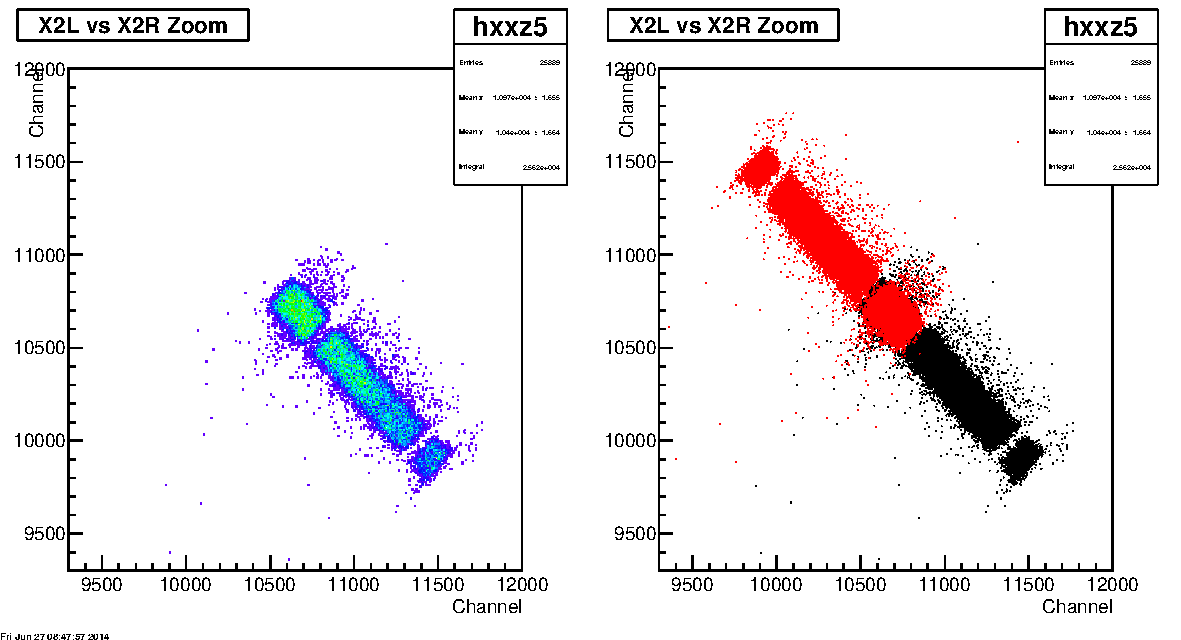
\includegraphics[width=\textwidth,keepaspectratio]{run00480_hxx5_reflect}
\caption{(Left) A plot of the signal X2L versus X2R.  By inspection, the correlation coefficient is approximately $-1$. Recall that XL signals correspond to the right-hand side of the detector (as viewed by the beam).  With $x=0$ defined as the left-hand side of the detector (as viewed by the beam), XR corresponds to the ``far'' signal. (Right) The plot from the left (black) is reflected (red) over the line $y=x$ as a visual test of gain-matching.}
\label{reflect}
\end{figure}
However, since the entire range of the detector is not illuminated, the reflection method only gives an approximate verification of the fit.  More significantly, the low dynamic range of the position signals 
(%the position signals 
covering $<1,280$ out of 40,960 channels) makes them very sensitive to the scaling parameter \verb|hxxcal[i][1]|.  Changes of 0.1\% in the scaling parameter will change the overlap of the reflected signals by several percent.  Therefore, a more sensitive calibration verification procedure is needed.
\subsection{Position Calibration}
\subsubsection{Method}
The relative positions of the features of the projection of the calibration mask are shown in Table~\ref{cal}.  What remains to be determined is the linear offset these features in terms of the relative position calculated using Eq.~\ref{detector_X}.  In order to determine the linear offset, and thus determine the calibrated detector position, the relative position of the gaps in the position spectrum need to be determined.  This is accomplished by fitting the position histogram with a piecewise-defined function.

\paragraph{Fitting the Peaks}
Traditionally, position calibration is accomplished by fitting known peaks in a spectrum.  In this test, the position spectra did not have peaks; rather they had wide regions illuminated by the scattered beam.  In order to attempt to fit these ``peaks,'' a nonconventional method was developed.
\vspace{0.5\baselineskip}
\par\noindent
\begin{minipage}{\linewidth}
\singlespace
\begin{lstlisting}
void lsload(Char_t *filename="cal/X1.lst")
{
  loadcal(filename);   
  ls1 = new TF1("ls1","([8]+[9]*x+[10]*x*x)*(x>(([0]-[7])/[6]))*(x<(([1]-[7])/[6]))+([8]+[9]*x+[10]*x*x)*(x>(([2]-[7])/[6]))*(x<(([3]-[7])/[6]))+([8]+[9]*x+[10]*x*x)*(x>(([4]-[7])/[6]))*(x<(([5]-[7])/[6]))");
  ls1->SetParName(6,"p6 range slope");
  ls1->SetParName(7,"p7 range offset");
  ls1->SetParName(8,"p8 fit offset");
  ls1->SetParName(9,"p9 fit slope");
  for(int i=0;i<6;i++){
    ls1->FixParameter(i,positions[i]);
    printf("i=%d positions[%d]=%5.1f parameter[%d]=%5.1f\n",i,i,positions[i],i,ls1->GetParameter(i));
  }
}  
\end{lstlisting}%
%\vspace{-1.0\baselineskip}
\end{minipage}
The function given in the code block above defines a polynomial over three ranges.  These three ranges correspond to the three ranges illuminated on each detector plane.  The quadratic function is explicitly defined in the \texttt{TF1} declaration as
\begin{equation}
\texttt{([8]+[9]*x+[10]*x*x)}
\label{eq:poly}
\end{equation}
instead of using the built-in ROOT function \verb|pol2| in order to force the fit parameters to be the same over each range.  This way, one function is fit to all of  the histogram data.  For calibrating the $x$-direction, the functional form of the Rutherford scattering cross section
\begin{equation}
\texttt{([8]+[9]*TMath::Power(sin([10]*x-[11]),-4))}
\label{eq:ruth}
\end{equation}
could also be used; however, the determination of the fit parameters using this equation are much less robust in ROOT as compared to fitting a histogram with a quadratic equation.  Furthermore, this form of the Rutherford scattering cross section only applies to $\varphi=0$.  Continuing with the quadratic fit, the range of the function may be defined in ROOT using the \texttt{TF1} constructor or it may be defined explicitly in the functional form.  In the above code block this is accomplished with the inclusion of the code segment \verb|*(x>a)*(x<b)| after each function definition.

By defining the function in this way, the range of the function may be an adjustable parameter.  The first six parameters of the function, which enter into the function via the range definitions, correspond to the calibration parameters shown in Table~\ref{cal}.  In the above code block, the calibration parameters are read in with the function \texttt{loadcal()} and then are made fixed in the \texttt{for} loop.  Parameters \texttt{[6]} and \texttt{[7]} are then the global slope and offset, respectively, of the known calibration parameters.  To aid in the fit, the variable parameters of the quadratic fit function (\texttt{[8]}, \texttt{[9]}, and \texttt{[10]}) can be measured on the central region only and then fixed.

The results of this technique are shown in Fig.~\ref{hxc_ls}.  This method is extremely sensitive to the initial values of the input parameters and is therefore both unreliable and ineffective. It also assumes \textit{a priori} knowledge of the position of the beam spot. In order to provide adequate input parameters for the fit, a robust and precise method was developed to locate the edges of the two ``valleys'' corresponding to the strips in the mask.

Figs.~\ref{hxc_ls} and \ref{hxc} are generated with a commands similar to the following.
\vsetroot
\begin{quote}
\begin{Verbatim}[firstnumber=0]
qfitc2mls("hxc2",87,141,3,"cal/X2.cal")
qfitc2mr("hxc2",87,141,3,"cal/X2.cal")
qfitc2mr("hxc3",13.1,40.8,3,"cal/Y2.cal")
\end{Verbatim}
\end{quote}
\vsetnone

\begin{figure}
\centering
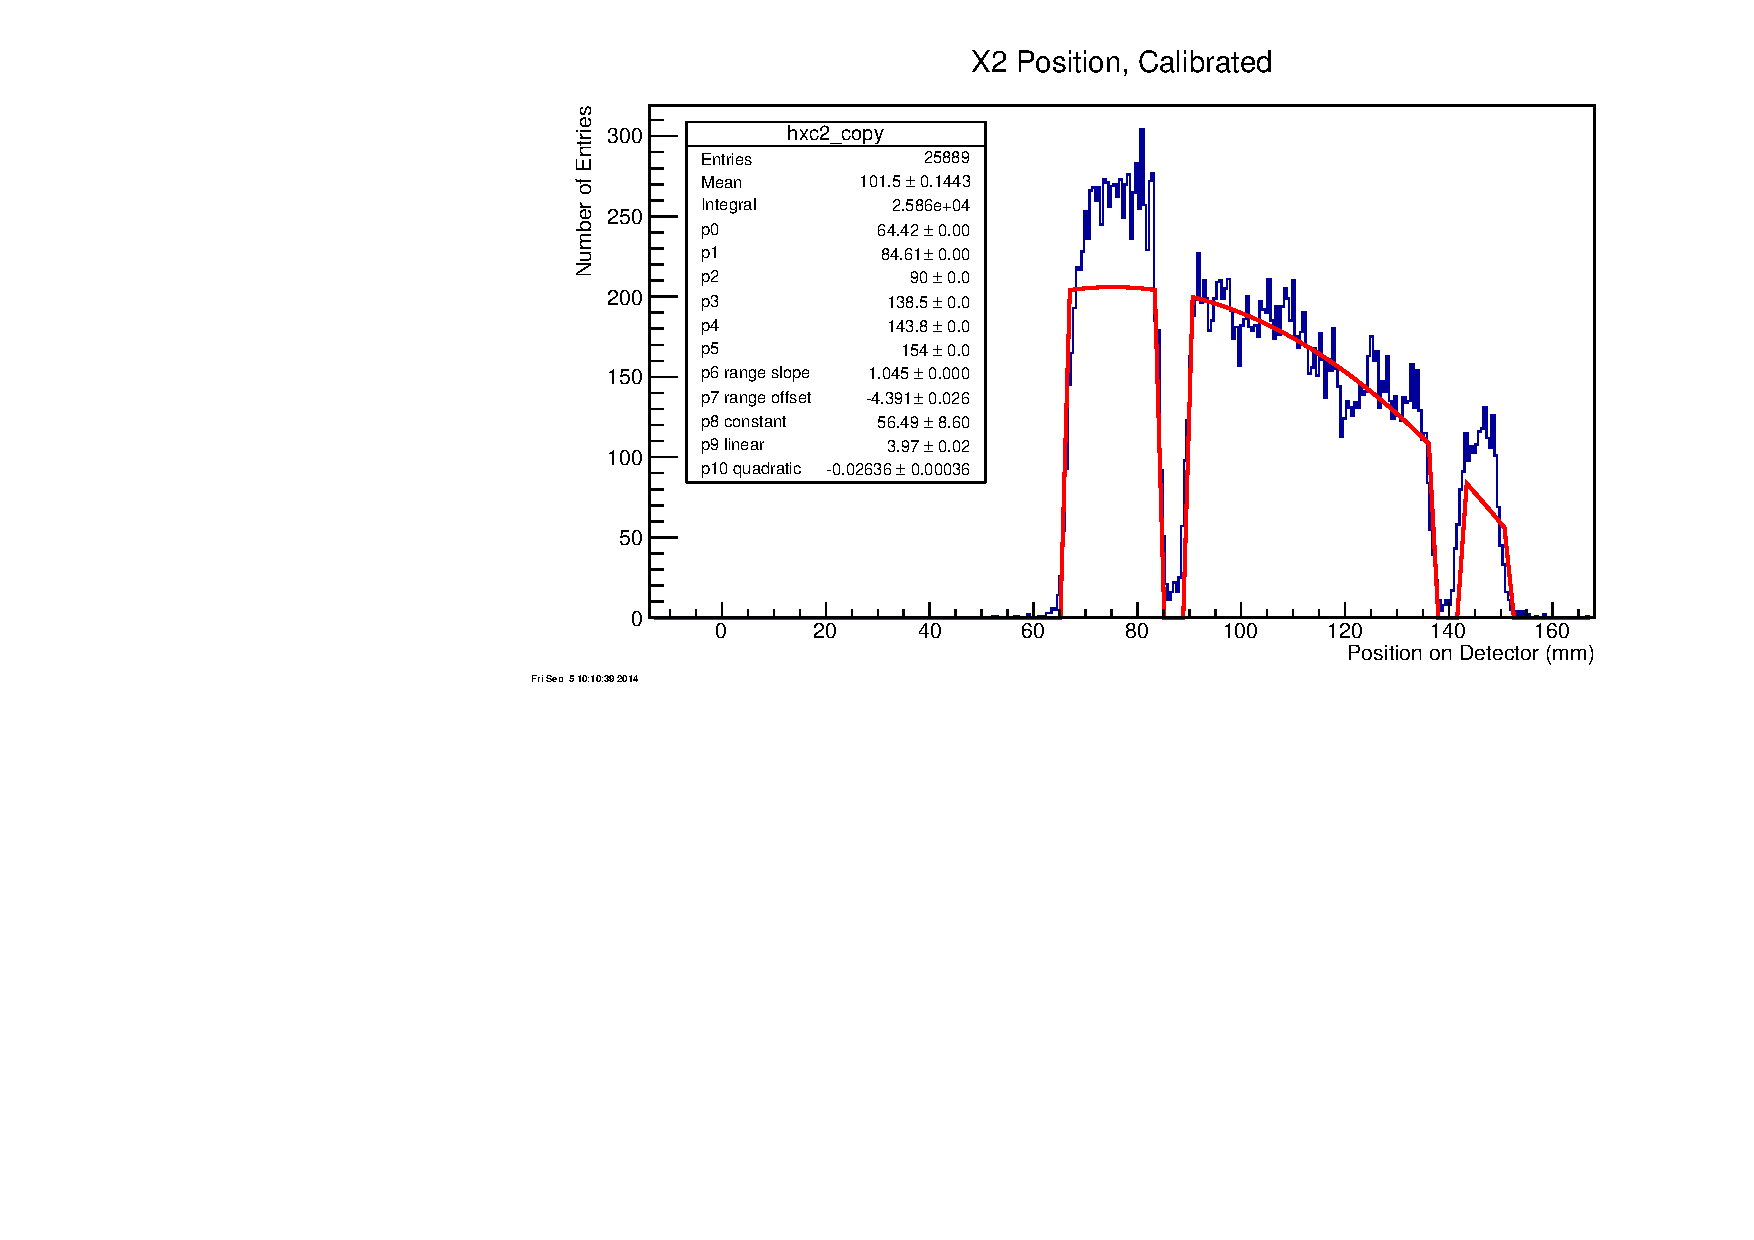
\includegraphics[width=\textwidth, keepaspectratio]{run_480_hxc2_ls}
\caption{Result of the fitting process by which the illuminated regions of the detector are fit.  The fixed relative positions of the edges of the illuminated region are fit to the ``peaks'' in the spectrum.}
\label{hxc_ls}
\end{figure}

\paragraph{Fitting the Valleys}
%Fitting the wide ``peaks'' in the spectrum is not very effective.  
Tables \ref{xpos} and \ref{ypos} provide 6 parameters with which to calibrate each of the the position spectra.  Including the outer edges of the illuminated region of the detector in the calibration procedure are dubious because the outer edges of the illuminated region are not sharply defined.  This is due to two effects.  First, the Kapton shields produce partial charge collection for trajectories at the edge of the detector.  This effect applies to both outer edges of the $y$-position spectra and the right-hand edge of the $x$-position spectra.  The second effect applies to the right-hand side of the $x$-position spectra.  This edge corresponds to the circular aperture of the mask, which does not provide a sharp cuttoff.

%Furthermore,
In addition to the uncertainty introduced by the edge effects outline above, the precise position of the outermost edges of the calibration spectra are not known \textit{a priori}. The parameters calculated in Tables \ref{xpos} and \ref{ypos} assume a point-like beam spot centered on the $z$-axis.  If the position of the beam spot is varied, the projected position of the mask will vary.  However, given that the $z$-position of the target, mask, and detector planes are fixed, the size and spacing of the gaps projected by the the vertical and horizontal strips of the mask are constant (at any given plane along the $z$-axis).

With these considerations in mind, the useful calibration parameters are limited to the central four edges.  By locating the center of each valley in the spectra, the relative position of all four calibration parameters can be determined with two fits. % (one for each valley). 
 This process is illustrated in Fig.~\ref{hxc}.  The data are scaled using the difference in the positions of the center of the gaps.  The scale factor is equal to the ratio of the known difference to  the measured difference. 
\begin{figure}
\centering
\hspace{\fill}
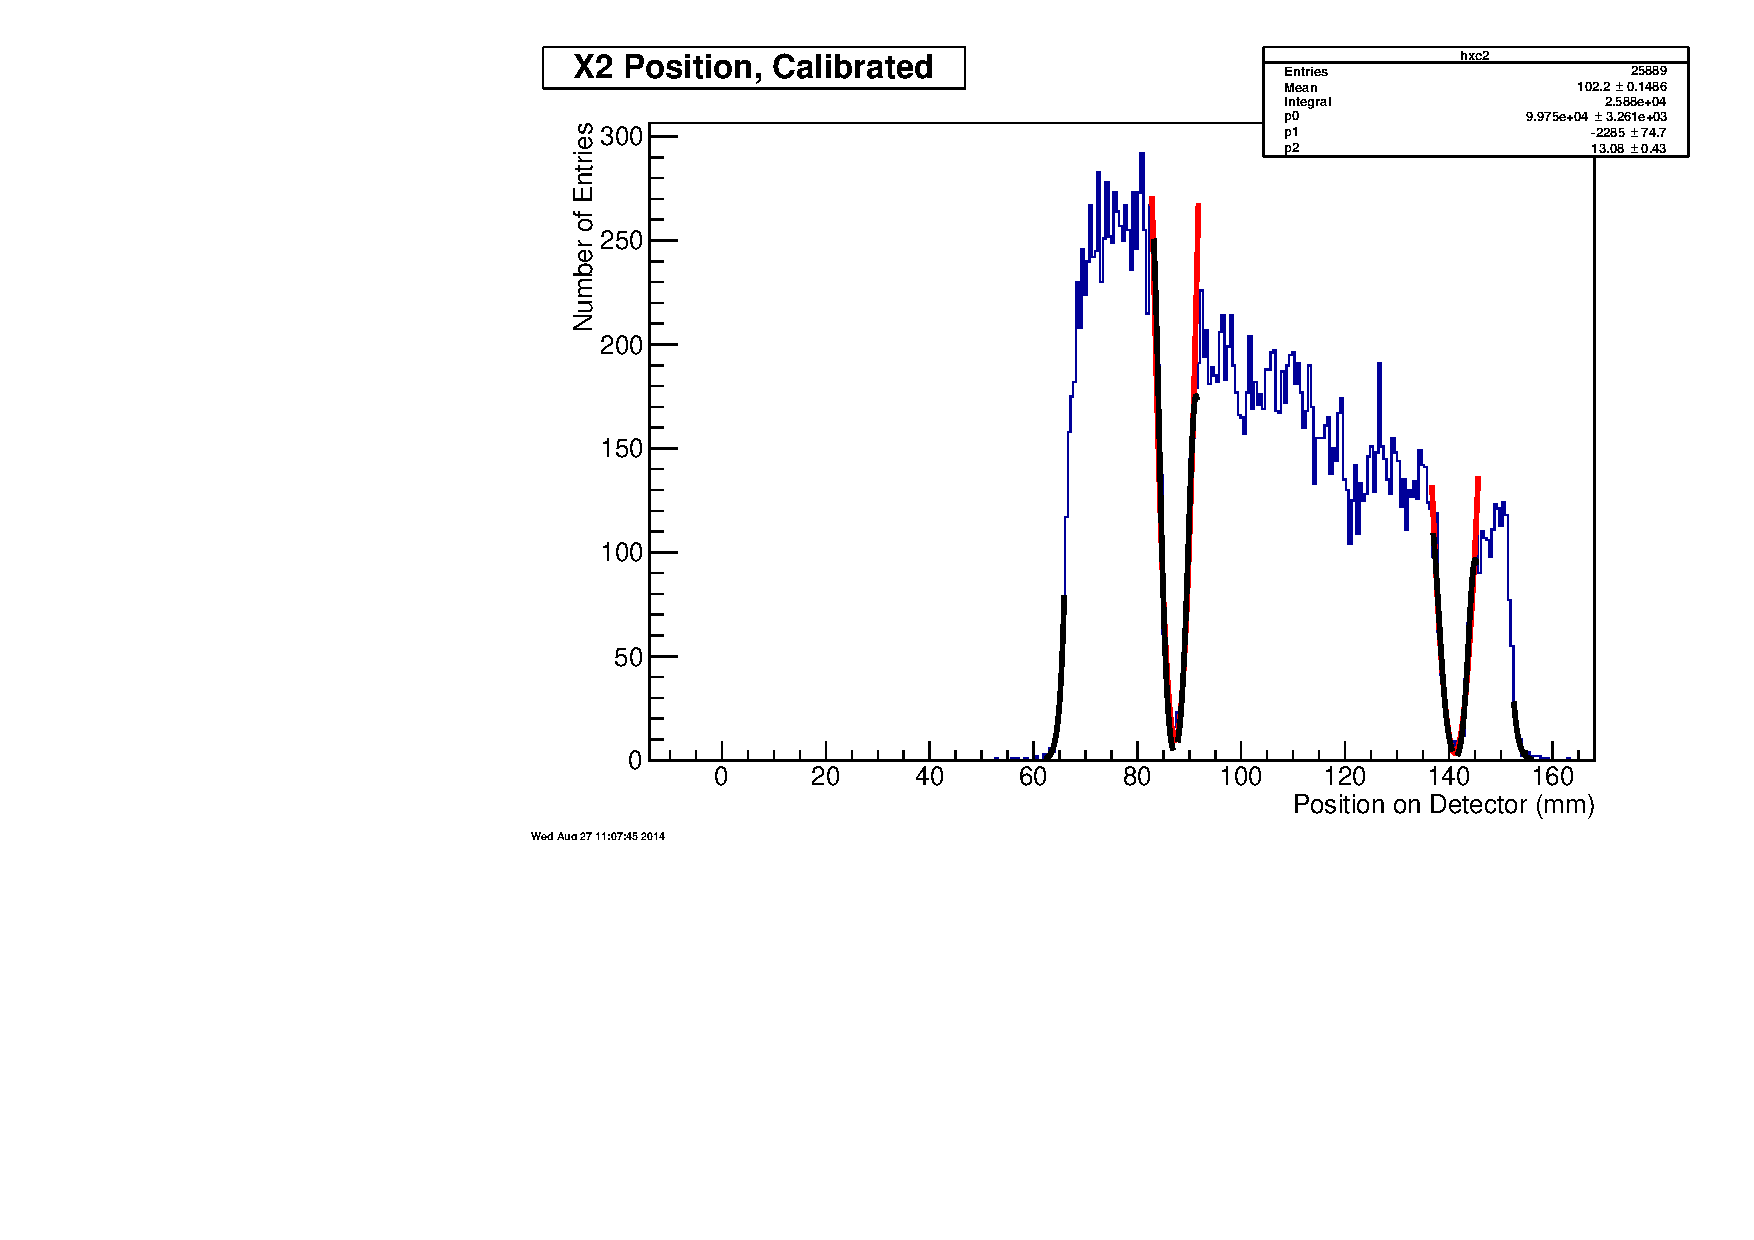
\includegraphics[width=0.48\textwidth, keepaspectratio]{run_480_hxc2}\hspace{\fill}
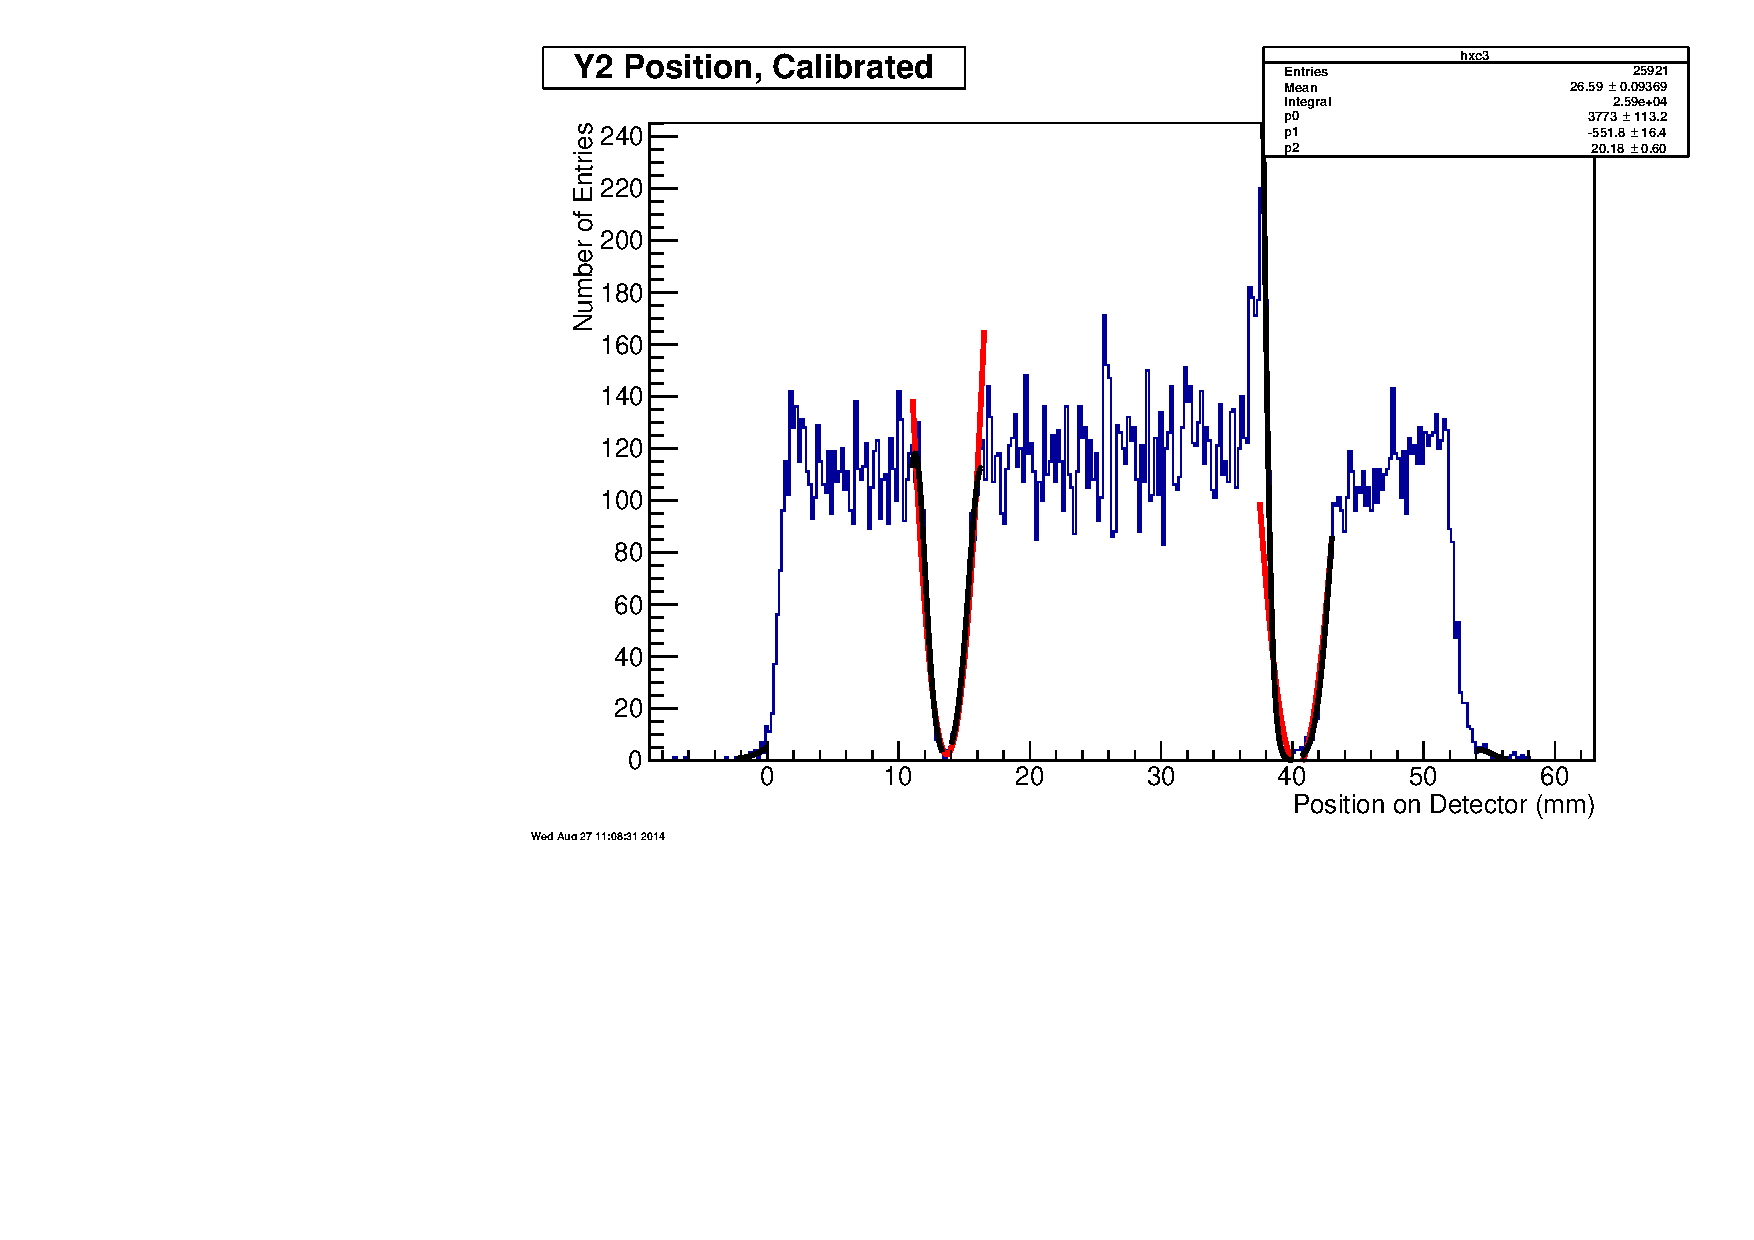
\includegraphics[width=0.48\textwidth, keepaspectratio]{run_480_hxc3} \hspace{\fill}
\caption{Position calibration technique.  Position X2 is shown on the left and position Y2 is shown on the right. The valleys between the illuminated areas of the detector are each fit with quadratic function (red lines) to locate the center of the gap.  The edges of the spectra are fit with gaussian functions (black lines) to determine the position resolution.}
\label{hxc}
\end{figure}

With this procedure, the position spectra are calibrated (in mm) based on the known detector geometry and independently of the $(x,y)$ position of the beam spot.  If the position of the beam spot is off-center, the position spectra are calibrated absolutely by the addition of a linear offset to correctly position the outer edges of the detector.  In the $y$-direction, this corresponds to centering the position spectrum. Fig.~\ref{yposreflect} shows the calibrated $y$-position spectra reflected with a given offset to align the edges.
\begin{figure}
  \centering
  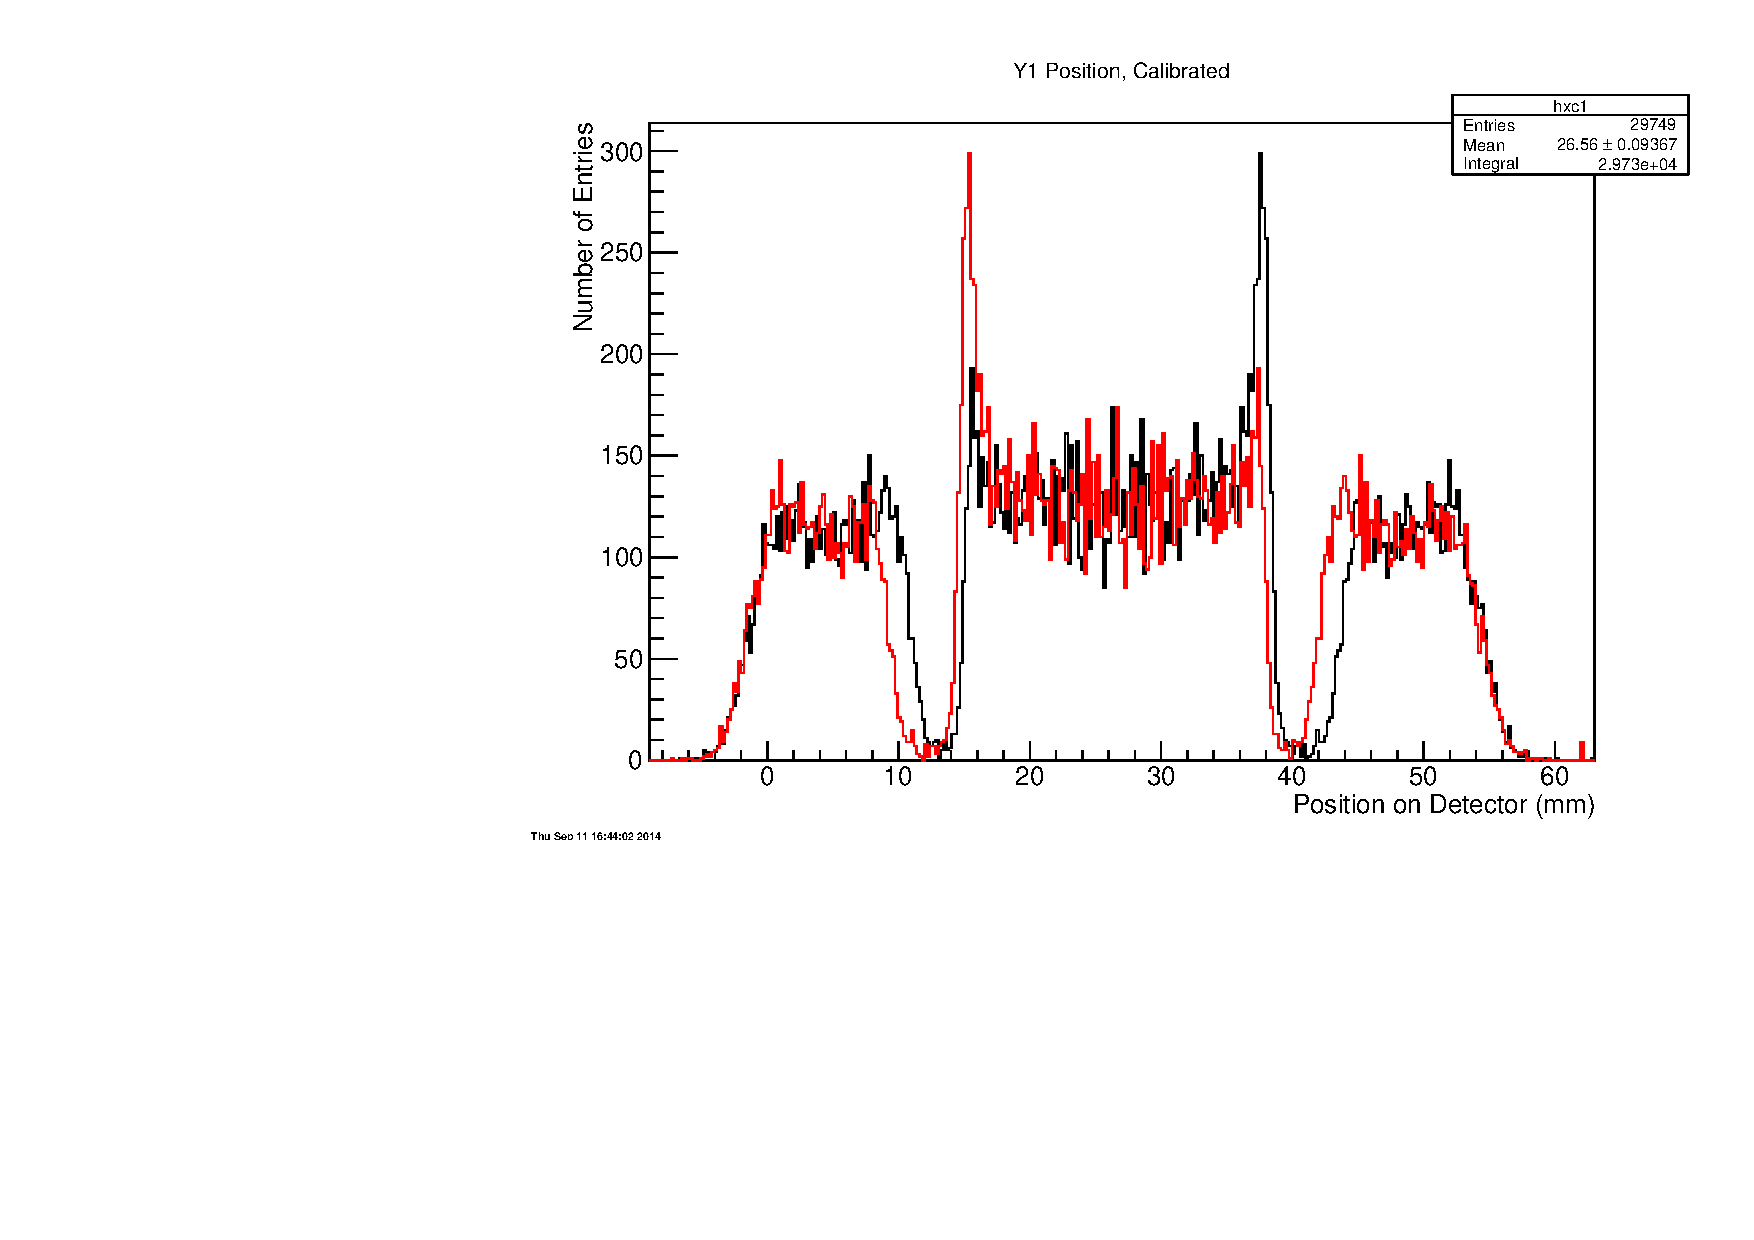
\includegraphics[width=0.48\textwidth,keepaspectratio]{run_480_hxc1_reflect}\hspace{\fill}
  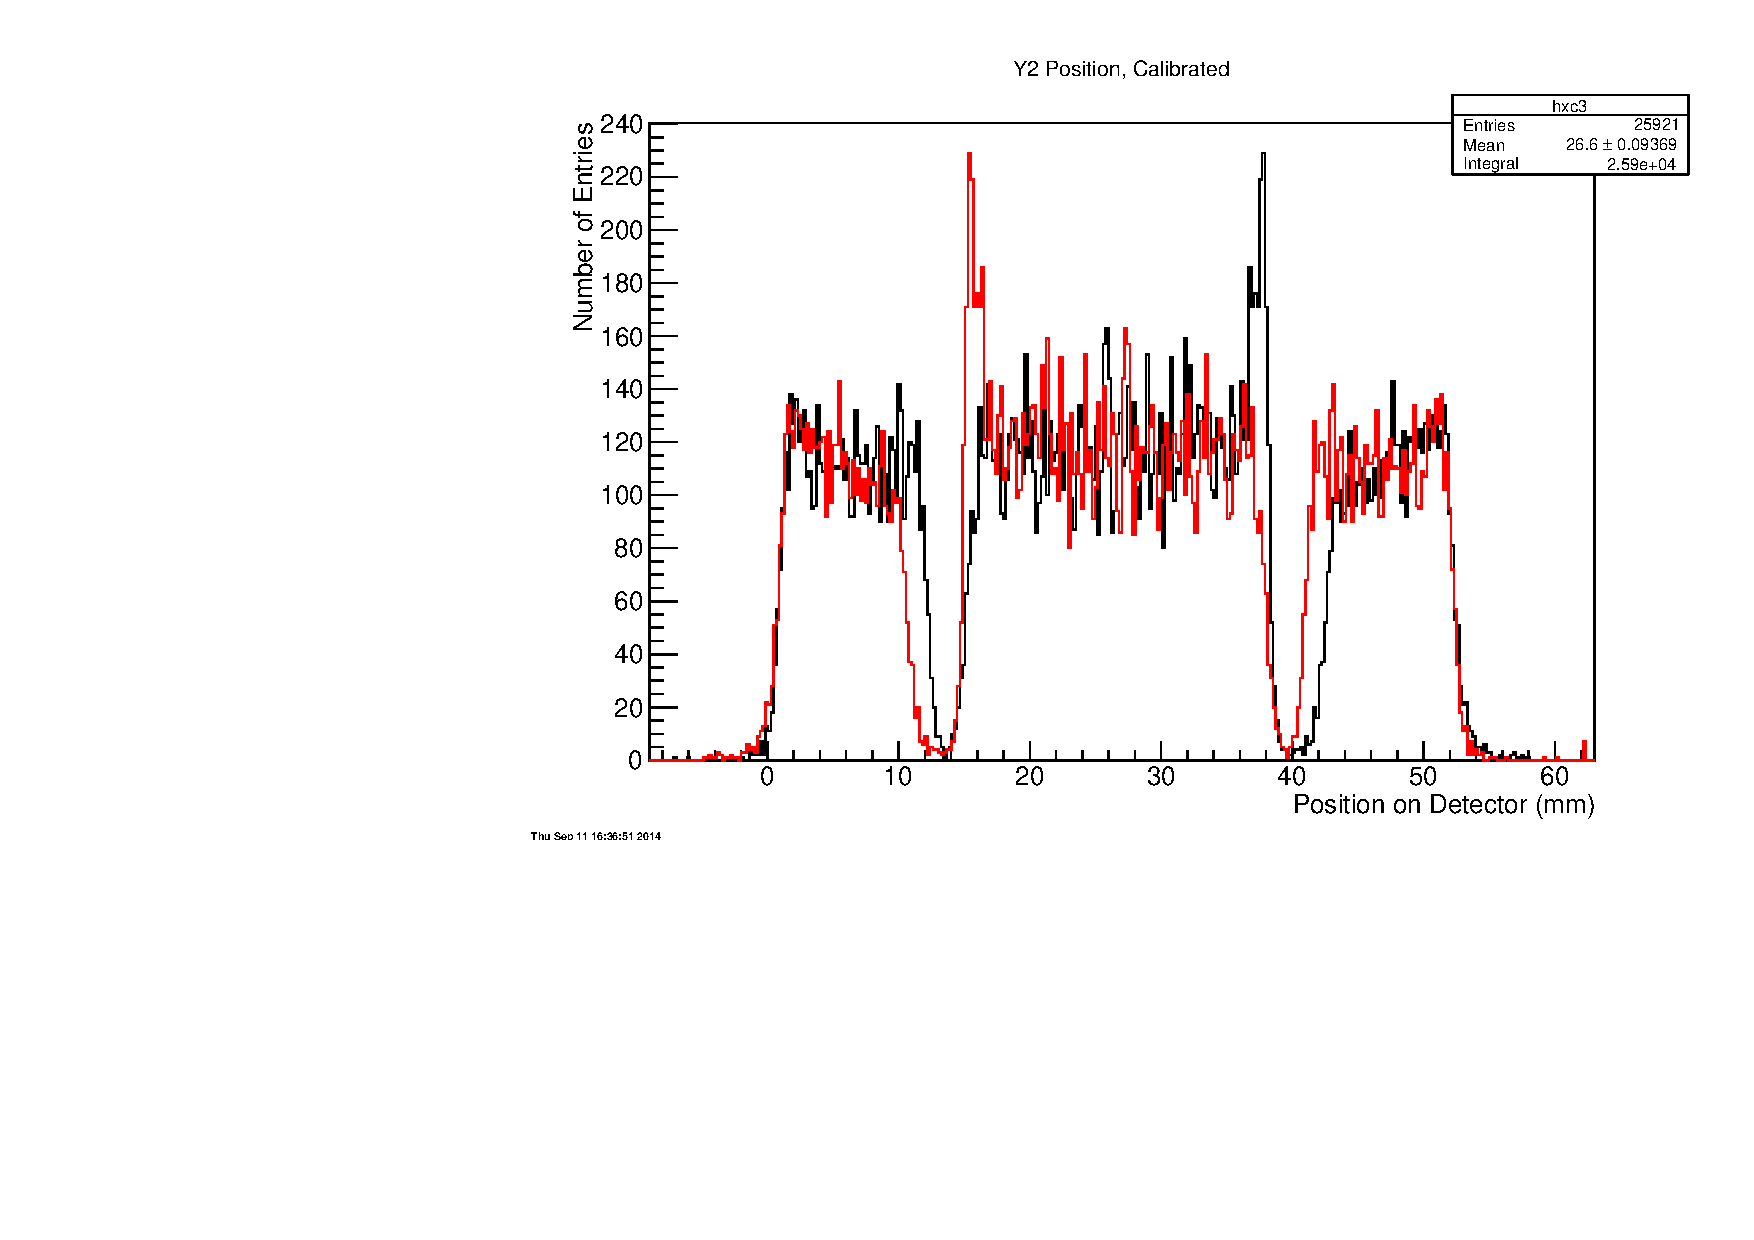
\includegraphics[width=0.48\textwidth,keepaspectratio]{run_480_hxc3_reflect}
   \caption{Calibrated $y$-position spectra (black) for each detector. The spectra have been reflected about the center of the detector and shifted (red) to align the outer edges of the spectra.  The Y1 spectrum has been shifted by 1.0\,mm and the Y2 spectrum has been shifted by 0.8\,mm.}
   \label{yposreflect}
\end{figure}
 %Calibrating the position spectra in this way provide a relative c
\subsubsection{Results}
The results of the valley fitting calibration procedure are shown for the $x$-positions in Fig.~\ref{htxc_x}.
\begin{figure}
\centering
\hspace{\fill}
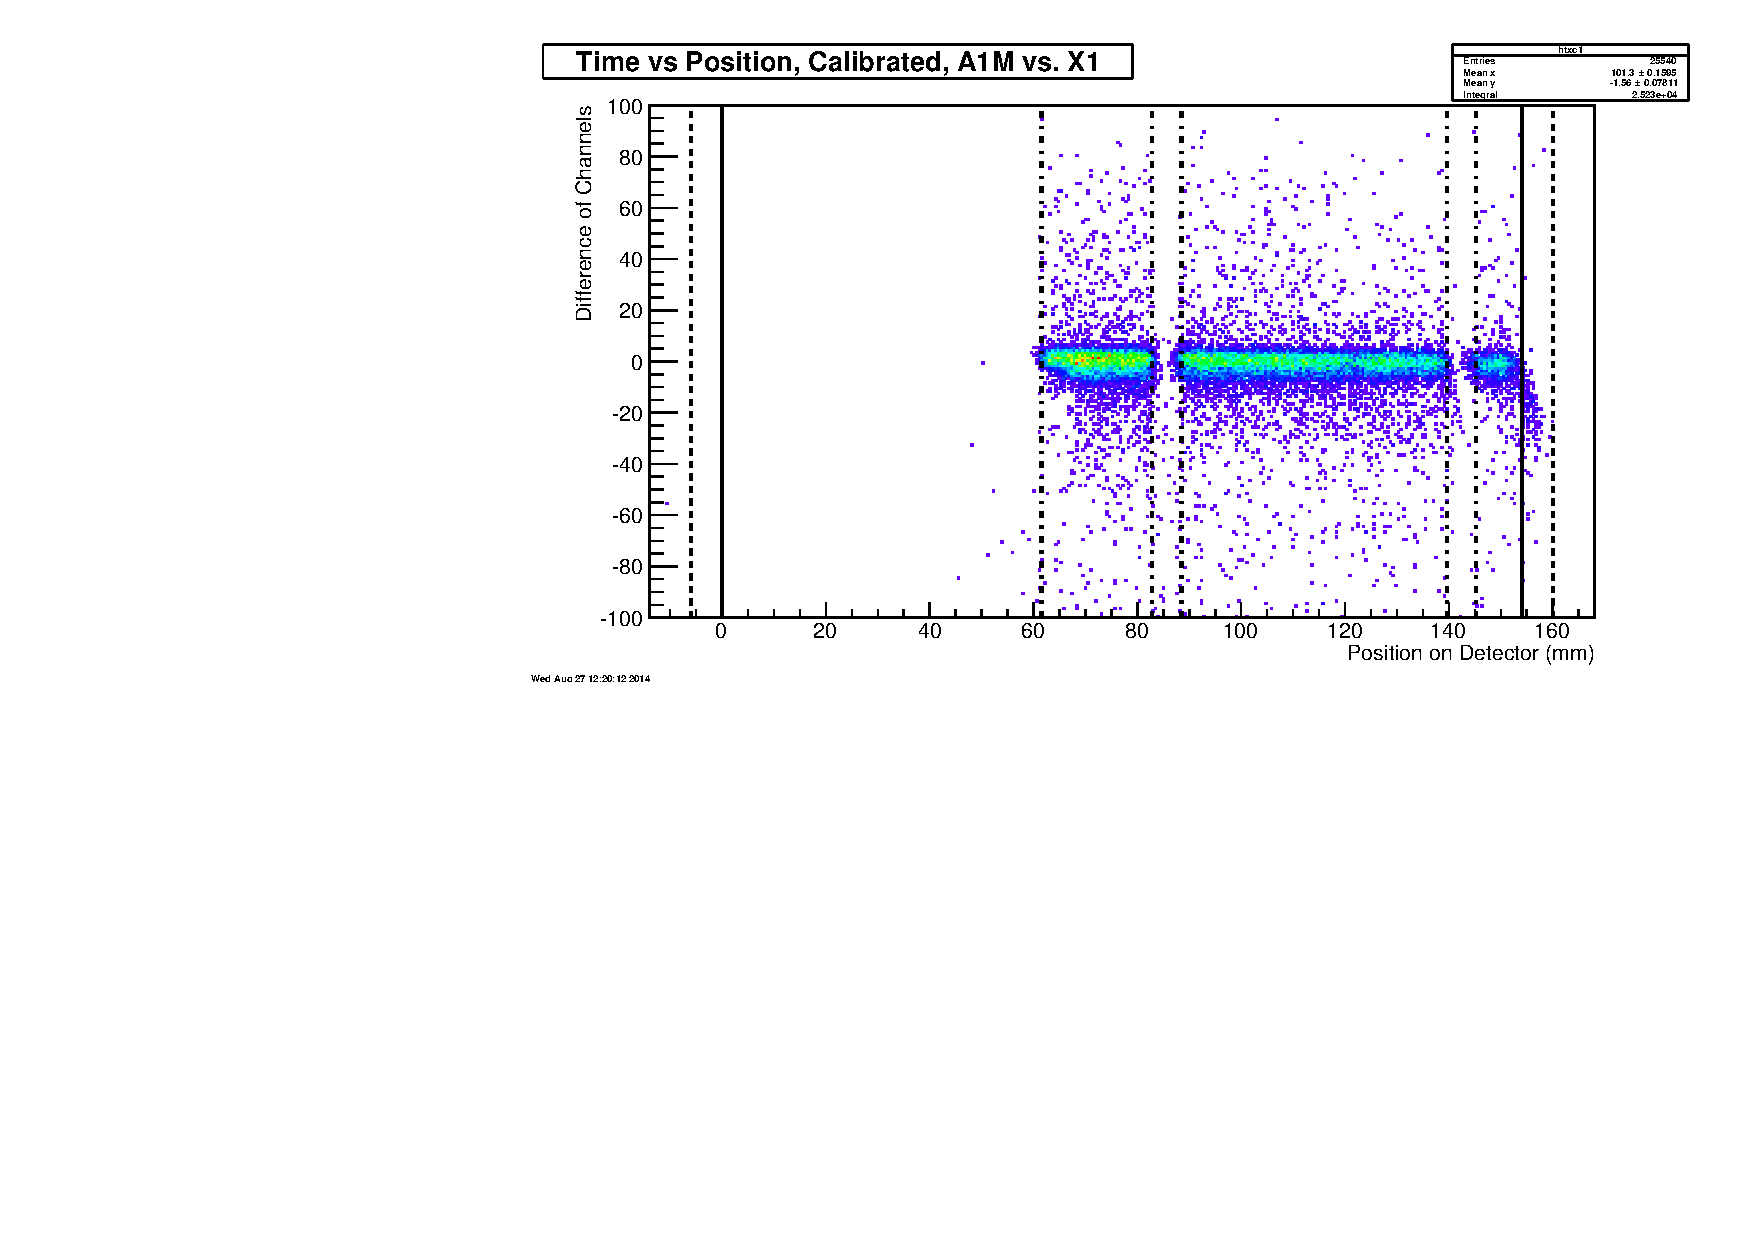
\includegraphics[width=0.48\textwidth, keepaspectratio]{run_480_htxc1}\hspace{\fill}
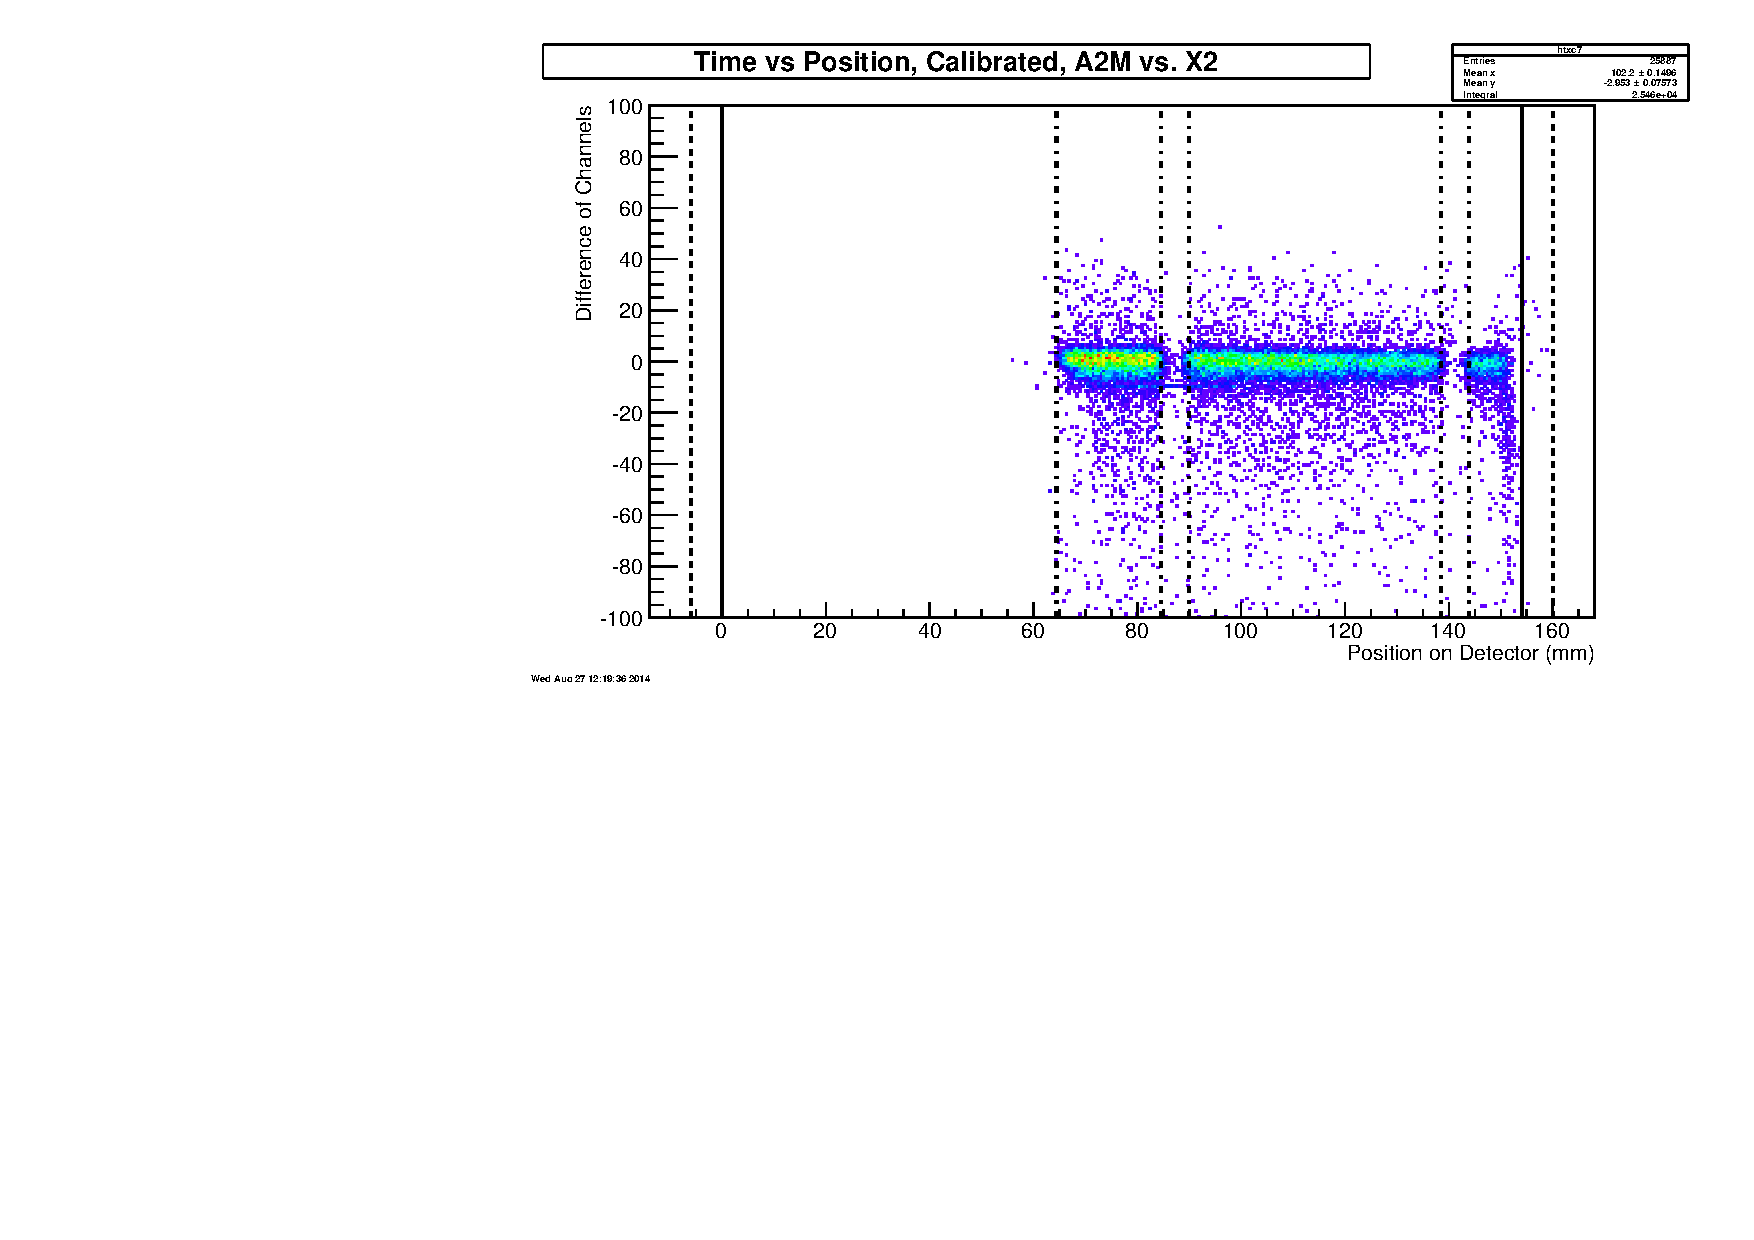
\includegraphics[width=0.48\textwidth, keepaspectratio]{run_480_htxc7} \hspace{\fill}
\caption{Difference in anode channel (time) plotted against calibrated $x$-position. The dashed lines indicate the edges of the detector.  The solid lines indicate the edges of the Kapton shields, corresponding to the edges of the fiducial area.  The dot-dashed lines indicate the projected position of the mask.  The cutoff in data at the right-hand side of X2 does not coincide with the edge of the fiducial area of the detector.  This may be due interference from the edge of the Mylar window (cf. Fig.~\ref{rays})}
\label{htxc_x}
\end{figure}
In order to determine the position resolution, the width of a known feature must be measured.  Usually this is done by measuring with width of peaks in spectra.  However, lacking any peaks, the edges in  the spectra can be used in similar manner.  The sharpness of the central edges of the position spectra provides a means by which to determine the position resolution.  The results of such an analysis are shown in Table~\ref{pos_res}.
\begin{table}[ht!]%
\centering
\begin{tabular}{c..}
\hline
\multicolumn{1}{c}{Edge}&\multicolumn{1}{c}{$\sigma$ (mm)}&\multicolumn{1}{c}{FWHM (mm)}\\ \hline \hline
%Edge & 3.974 & FWHM\\
1 & 1.43&3.36\\
2 & 1.48&3.49\\
3 & 1.68&3.95\\
4 & 1.19&2.79\\
Average & 1.44&3.40\\
\hline
\end{tabular}
\caption{Calibrated position resolution for position X2.}
\label{pos_res}
\end{table}
The resolutions presented in Table~\ref{pos_res} represent the cumulative effect of multiple contributions. Some of the possible contributions to the total measured position resolution are as follows.
\begin{itemize}
  \setlength{\itemsep}{0pt}
\setlength{\parskip}{0pt}
\setlength{\parsep}{0pt}
  \item The intrinsic detector resolution.
  \item The transverse extent of the particle trajectories.
  \item The position, extent, and distribution of the beam spot.
  \item The effect of beam scattering off of the mask.
\end{itemize}
%The transverse extent of the particle trajectories tend to smear out the position. In addition to the intrinsic detector resolution,
In order to determine the intrinsic position resolution of the detectors the other contributions to the measured resolution need to be deconvoluted.  The is accomplished with simulations.
\subsection{Simulations}
A Monte Carlo simulation has been constructed to study the various contributions to the measured resolution.  An example output is shown in Fig.~\ref{sims}. To produce the figures discussed in this section, the simulation included a uniform spherical scattering distribution and a finite beam spot.  Specifically, the beam spot has been simulated as a symmetric Gaussian distribution with 90\% of the beam falling within a radius of $\rho=1.0$\,mm ($\sigma = 0.608$\,mm). This beam spot size was selected to be conservatively large and yet physically reasonable.
\subsubsection{Contributions}
One of the purposes of studying the detector via a simulation was to deconvolve the various contributions to the detector resolution. The results of the simulation study indicate that the observed detector resolution is dominated by the intrinsic detector resolution.  As discussed in Section~\ref{cal_def}, the contribution of the transverse extent of particle trajectories is less than 170\,$\mu$m at the edges of the detector. Near the center of the detector, the contribution approaches zero. These effects are neglected in all of the simulations.

To isolate the contribution of the beam spot size, simulations were run neglecting the effects of beam scattering and detector resolution. Fig.~\ref{sims} shows the simulated position spectra from detector 2.  Comparing Fig.~\ref{sims} with Fig.~\ref{hxc}, one sees that the beam spot size has a minimal contribution to the measured detector resolution. This is not surprising given the distance between the target and the detectors (682.9\,mm) and reasonably-assumed size of the beam spot (1--2\,mm). In order to reproduce the observed resolution in Fig.~\ref{hxc} from the contribution of the beam spot alone, physically unrealistic beam spot sizes are required. For example, a beam spot greater than the size of the target foil is required.
\begin{figure}%
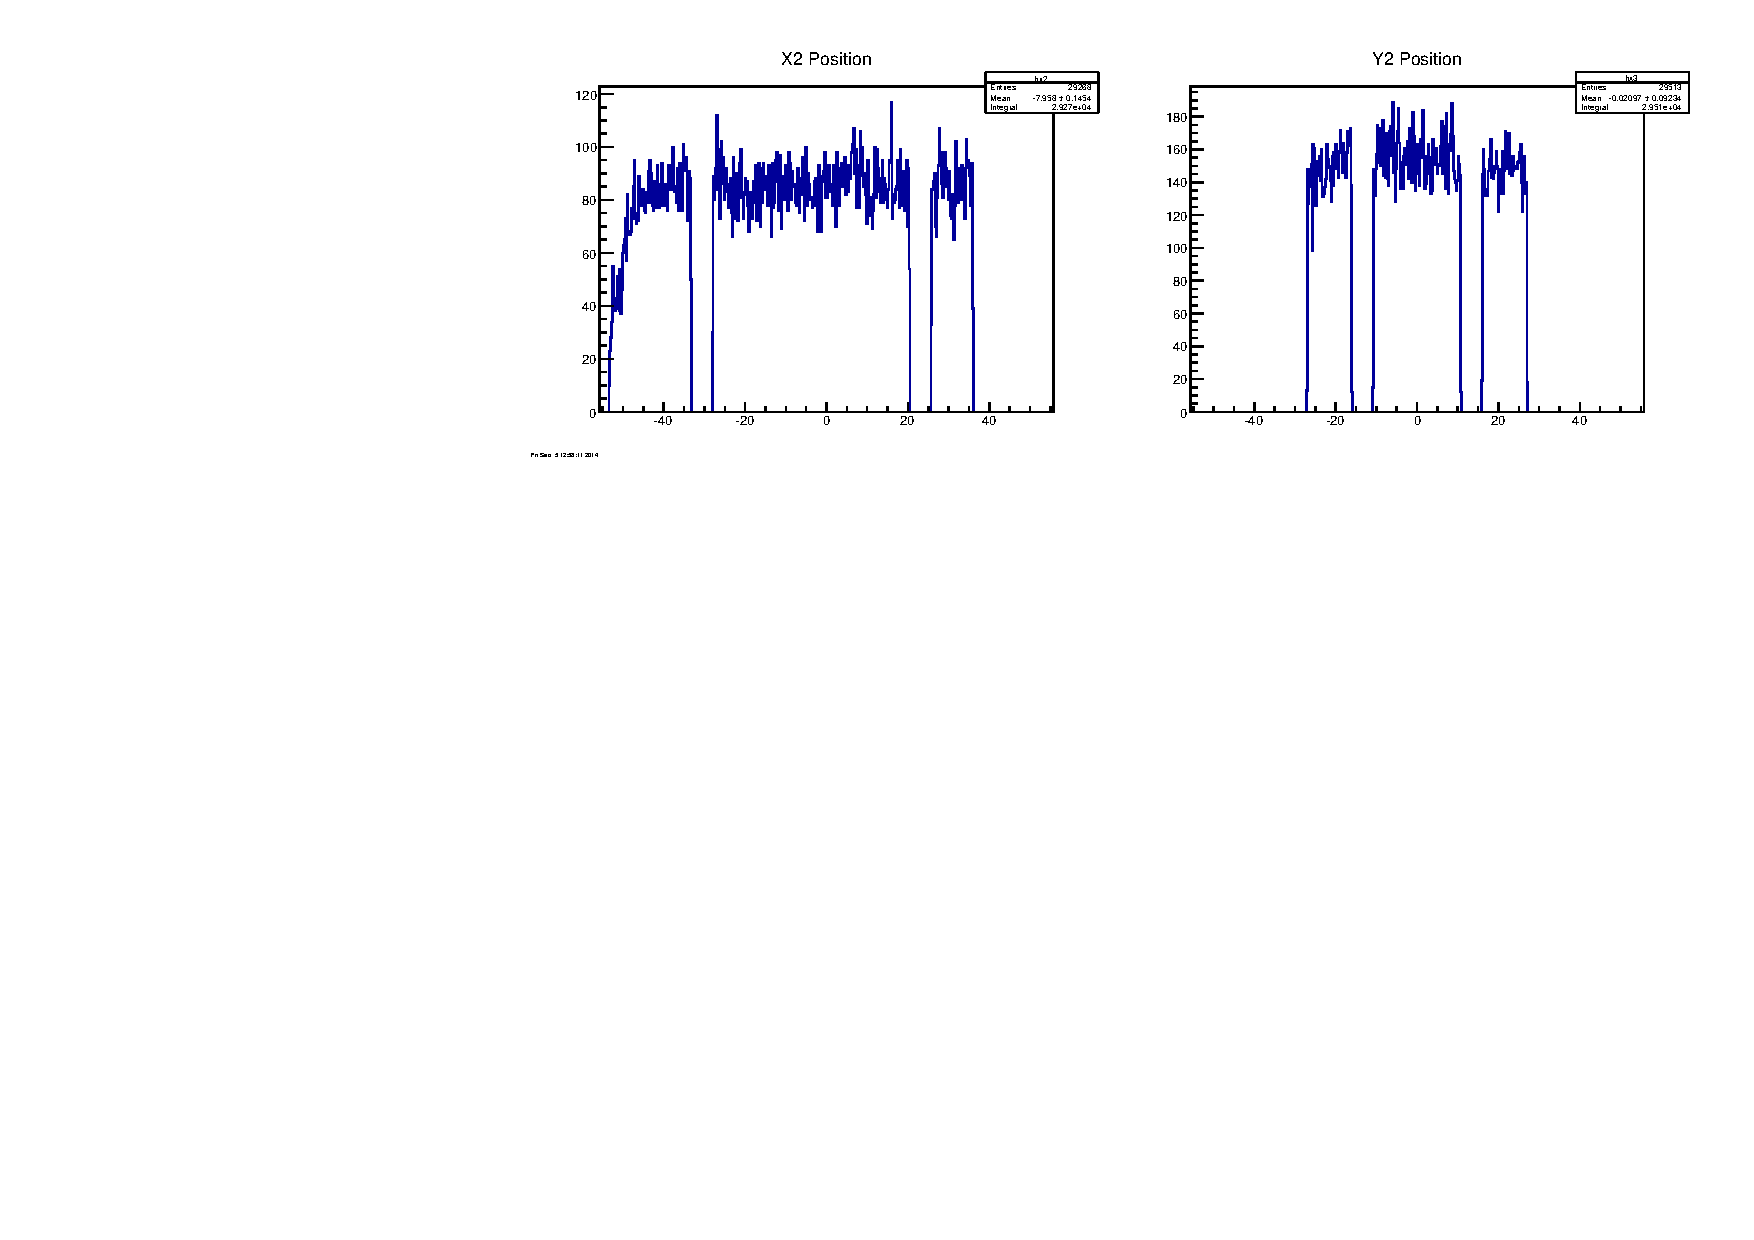
\includegraphics[width=\columnwidth]{sims}%
\caption{Simulated positions spectra of detector 2.}%
\label{sims}%
\end{figure}

\subsubsection{Fitting the Data}
The determination of the detector resolution is accomplished by fitting the data with the simulation. The position of the beam spot is accounted for by geometrically aligning the features of the simulation with those the data. Once the simulation is aligned to the data, the measurement resolution of the simulation is varied to match the shape of the data. Fig.~\ref{sim_comp} show the result of fitting the data with the simulation in order to determine the position resolution of the detector. Because the simulation adequately reproduces the data without including edge scattering, implementation of that effect is neglected. In this example, the data was best fit with a simulated intrinsic detector resolution of 1.3\,mm (3.06\,mm~FWHM).  This fit is consistent with the dubious edge-fitting method presenting in the previous section. For an example such as this, where the wires are not resolved, the quality of the fit of the simulation could be improved on the order of 8\% by including a realistic angular distribution.
\begin{figure}%
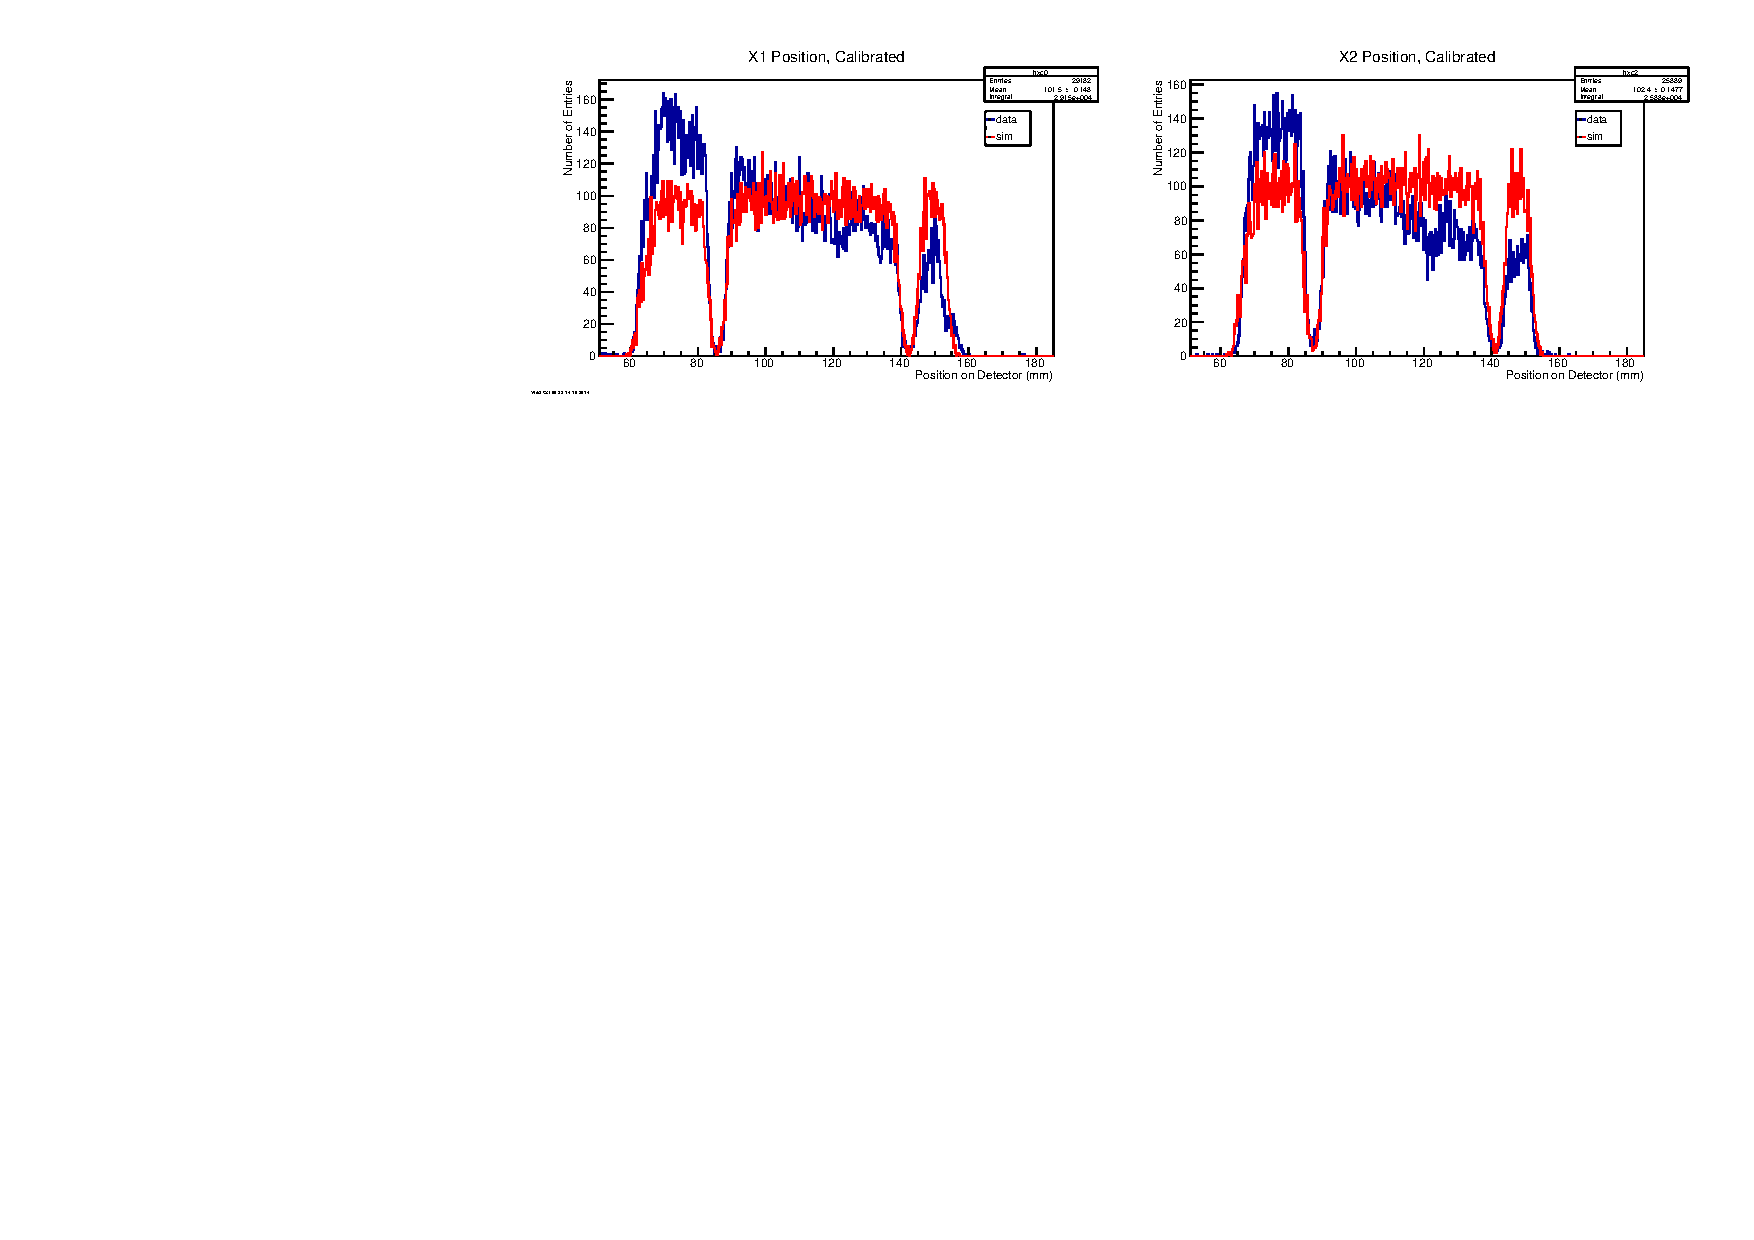
\includegraphics[width=\columnwidth]{run_480_compX}%
\caption{Simulated and measured $x$-position spectra of for each detector. The data (blue) have been fit with a simulated spectra using the following assumptions: a 1.43\,mm~FWHM beam spot centered at the origin and a detector resolution of 1.3\,mm (3.06\,mm~FWHM).}%
\label{sim_comp}%
\end{figure}




